\chapter{Experiments}\label{ch:tests}
When working on a field where human perception plays a significant role, it is important to test whether your work makes sense for target users and if it solves successfully the problem that was designed for.

To examine the immersion of real-time produced and physics-based sounds on game players, we performed \textit{MUSHRA}\cite{series2014method} tests to people. Our aim was to answer the following questions: \begin{inparaenum}[1)]
\item Which of the two synthesis methods (sinusoidal and filter-based additive synthesis) is closer to reality? 
\item Does physics-based synthesis make a sound more realistic and less boring?
\item Which is the range (in Q-factor values) of every material's sound?
\end{inparaenum}.
The results of the experiments are used to verify the modal synthesis methods implemented in this thesis, choose the more qualitative one and increase our understanding of spectral characteristics in relation with the material of the object. 

\section{Preparation}
For the experiments we used several audio files that we recorded inside the Unity\textsuperscript{\textregistered} platform. We designed two special scenes for this purpose, because we wanted to test both the impulse response of the synthesis model and the sounds in real-life conditions -when an object is falling and colliding with other objects (figure \ref{fig:test_scenes}). 

\begin{figure}[H]
    \centering
    \begin{subfigure}[b]{0.45\textwidth}
        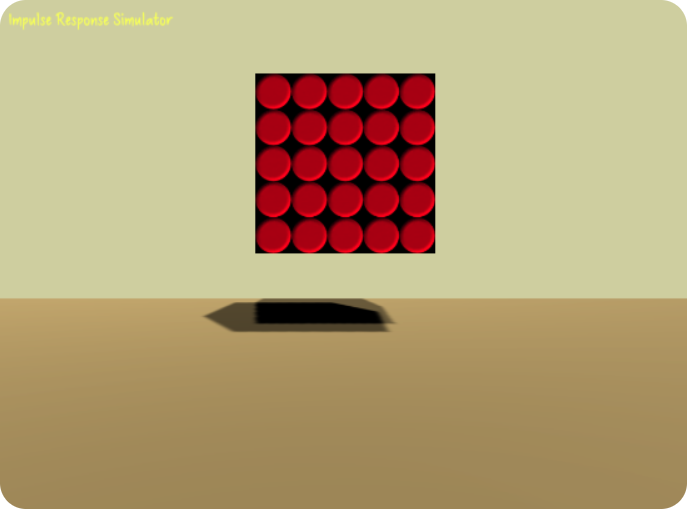
\includegraphics[width=\textwidth]{impulsescene_r.PNG}
        \caption{Impulse Response Simulator Scene.}
        \label{fig:test_sc1}
    \end{subfigure}
    ~ %add desired spacing between images, e. g. ~, \quad, \qquad, \hfill etc. 
      %(or a blank line to force the subfigure onto a new line)
    \begin{subfigure}[b]{0.45\textwidth}
        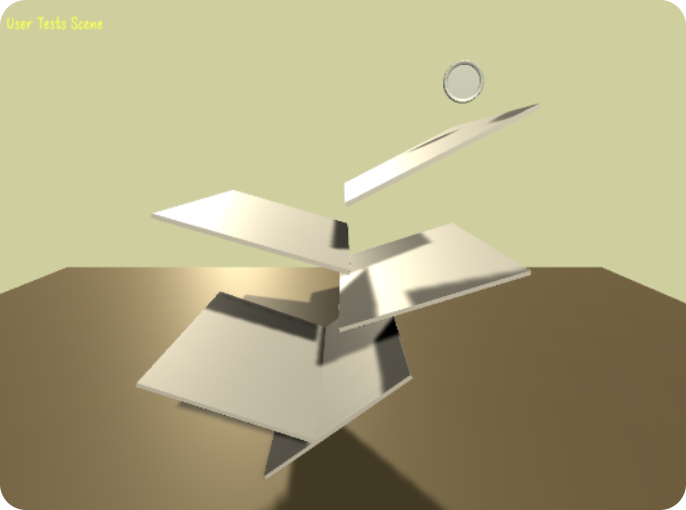
\includegraphics[width=\textwidth]{usertestscene_r.PNG}
        \caption{Real-Life Conditions Scene.}
        \label{fig:test_sc2}
    \end{subfigure}
    \caption{The Unity\textsuperscript{\textregistered} Scenes designed to record the audio files used for the user tests.}\label{fig:test_scenes}
\end{figure}

In the first scene (figure \ref{fig:test_sc1}), we recorded the audio files for the first experiment. During the recording session, we ``tagged'' the cube as different objects (a process that assigns to the cube different modal data) and let it touch the ground without any bounce. We also repeated the process with an Audio Source and the recordings files, to achieve consistency of the stimuli.

In the second scene (figure \ref{fig:test_sc2}), we recorded the audio files for the second and third experiment. In this scene, objects fall, roll and scratch freely on rotated platforms, simulating a real room with obstacles.

Every sound in the audio files starts 1 second after participant presses play and ends half a second after no sound can be heard. They are recorded with 16-bit resolution and a sample rate of 44100Hz using Audacity\textsuperscript{\textregistered} \cite{bib:audacity}.

\section{Stimuli}
We performed three different tests. In the first test, the participant listens to 44 impulse responses, corresponding to different areas of the eleven materials. Each trial of the test includes a reference sound, which is the recording of the actual sound produced by the physical object and the two different synthesized sounds, corresponding to the two examined methods. He is then asked to choose which of the two synthesized sounds is closer to the reference and whether it is very or less close. The goal of this experiment was to gather information about the quality of the two methods and addresses the best of the two.

In the second test, the stimuli consists of 33 trials that contain sounds produced by falling objects. Each trial includes one sound that is produced when object is split into ``sound areas'' and each area produces a different sound and a second sound that is produced when every point of the object makes the same sound. This single sound was chosen to be the one produced from the area of each object where the recording taken (section \ref{sec:recordings}) was the closest to the real sound in our opinion. Participants were asked which of the two they preferred and how much in a scale from ``A is the same as B" to ``A is much better than B". This test provided us with the immersion results of sound variation within one object.

The stimuli of the third test are sounds coming from five different objects, one of each material under testing (plastic jug, wooden mortar, ceramic plate, glass bottle and metallic cooking pot). For each object, we use 10 different sounds for each of the two synthesis methods. Each trial includes 10 sounds that correspond to the same event, but with a small variation on the Q-factor for every sound. More specifically, starting from a value of 1000, we increased the Q-factor by 200 up to 4600, removed some sounds that were too similar with others to decrease the size of the test and provided participants with the rest. They were asked to choose the sounds where, in their opinion, a change in the material happened. We performed this test to validate the chosen values for the Q-factor.

In the two first experiments, both the sequence of trials and the conditions (which method is A and which is B) are randomized. However, in experiment number three, we wanted to keep an increasing habit on the Q-factor, otherwise it would not make sense. Hence we randomized only the sequence of the trials.

Stimuli was presented to the participants through a pair of \textit{AKG K271} headphones, in a room with reduced external noise.

\section{Participants}
\Todo{number of participants, age, gender, normal hearing, job}
The participants are three adult volunteers. Zero women and three men, aged $25$ to $30$. Their mean age is $27$ with a standard deviation of $2.16$. They stated normal hearing. They have different backgrounds, namely a Digital Signal Processing (DSP) engineer, a mathematician and a movie director.

\section{Test Results}

\subsection{1st Experiment}
Results of the 1st experiment are shown in figure \ref{fig:test1}. We divided the results into smaller sub-graphs, one for each of the eleven objects, to examine the participants' preference in the synthesis methods per object. Particularly, their opinion on which of the two resembles more the original recording of the real-world object (used as reference).

\begin{figure}[H]
  \centering
    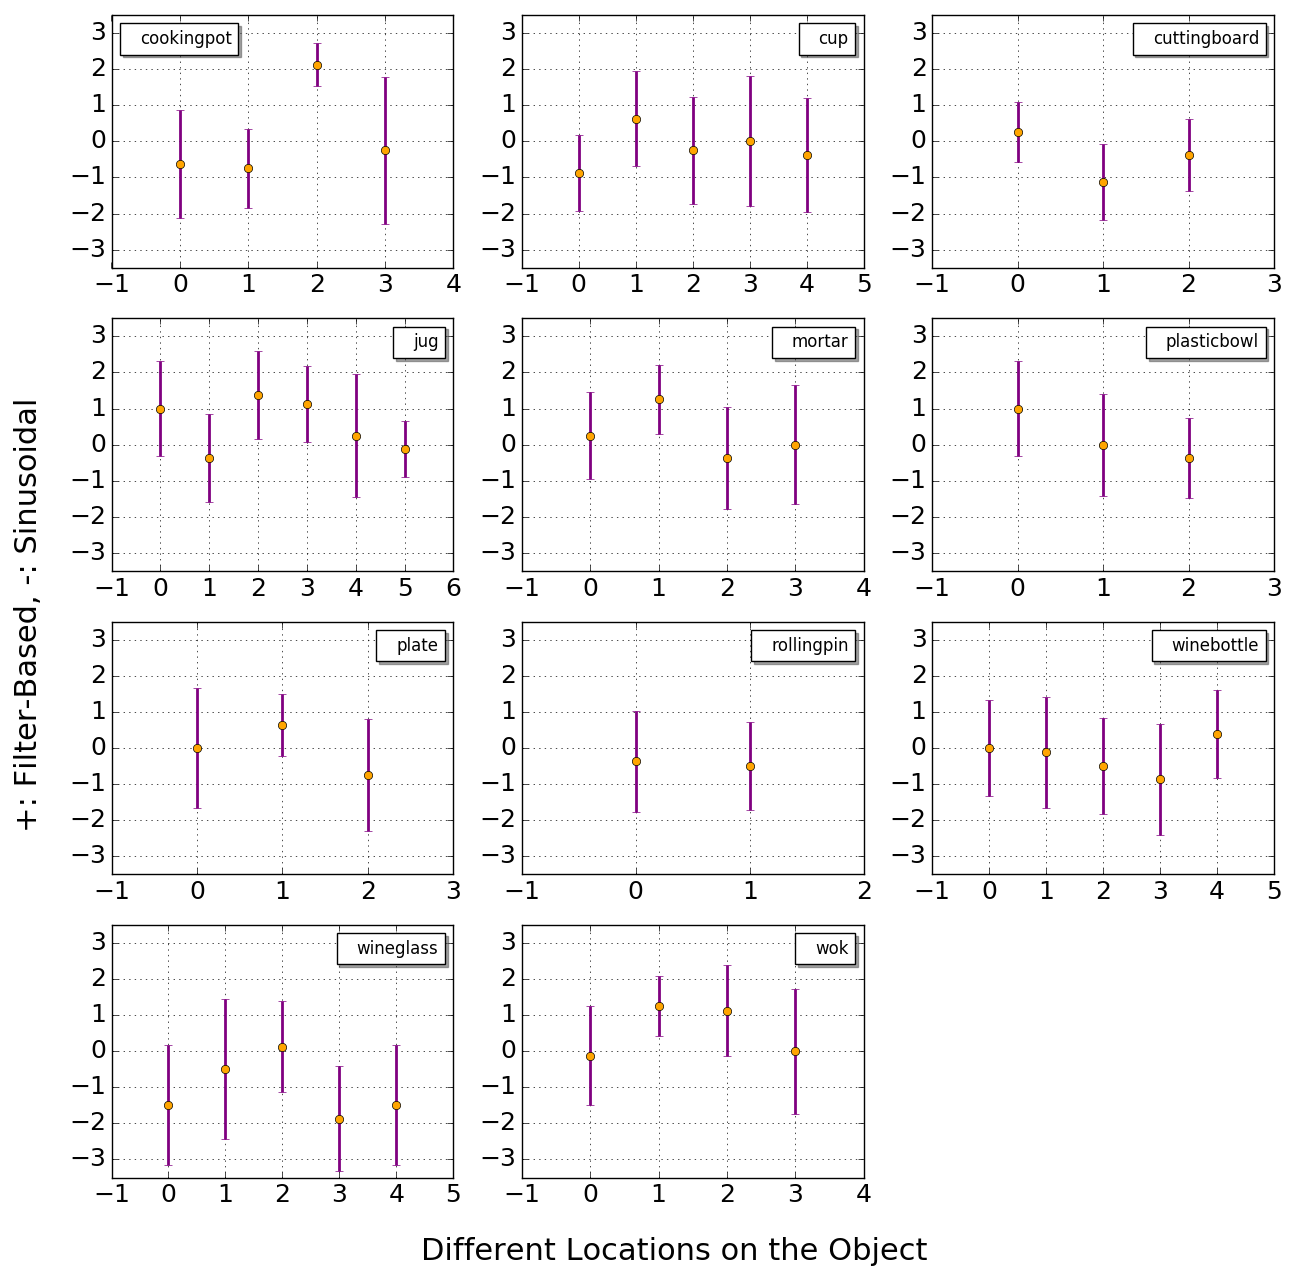
\includegraphics[width=\textwidth]{test1.png}
      \caption{The mean values and standard deviations per location for all objects. Positive values give a preference to the filter-based method, while negative ones give preference to the sinusoidal method. Participants choises were 0: both sound the same, 1/-1: the chosen is slightly better, 2/-2: the chosen is better and 3/-3: the chosen is much better.}\label{fig:test1}
\end{figure}

Participants were asked to move a slider between the integer values $-3$ and $3$. Positive values correspond to a preference in the filter-based method, negative in the sinusoidal method and zero values means that both methods sound the same. Possible answers are displayed in table \ref{tab:test1_ans}. Every different tick of the x-axis corresponds to a different ``sound area'' of the object. From left to right the areas go from the top to the bottom.

\begin{table}[H]
	\centering
    \begin{tabular}{ c  c  l  }
    \toprule
    \textbf{Slider value} & \textbf{Method} & \textbf{Amount of Preference} \\ \toprule
    \addlinespace
    $3$ & Filter-based & Much better  \\
    $2$ & Filter-based & Better \\
    $1$ & Filter-based & Slightly better \\ 
    \addlinespace
    $0$ & \multicolumn{2}{c}{Both sound the same} \\
    \addlinespace
    $-1$ & Sinusoidal & Slightly better \\ 
    $-2$ & Sinusoidal & Better \\ 
    $-3$ & Sinusoidal & Much better \\
    \addlinespace
    \bottomrule
    \end{tabular}
    \caption{Possible answers for the 1st experiment.}
    \label{tab:test1_ans}
\end{table}  

With this test we wanted to answer the question of which of the two synthesis methods - filter based or sinusoidal additive synthesis - used in this thesis is better. From figure \ref{fig:test1} we can see that one universal answer for all objects does not exist. For example, we can see a tendency for the filter based method for the plastic (jug and plastic bowl) and the metal (cooking pot and wok) objects, but there is no distinct result for the rest of the objects.

\Todo{check if those still are valid after adding more participants.}

\subsection{2nd experiment}
For the second experiment we also divided the results into sub-graphs per object. They are presented in figure \ref{fig:test2}. This experiment examines the participants' preference between a sound variation on impact sounds depending on the hit point and a single impact sound per object.

Participants were asked to use a slider similar to the previous test, with possible answers shown in the table \ref{tab:test2_ans}. Positive values correspond to preference in sound variation, while negative ones correspond to preference in single sound per object. The three different ticks on the x-axis correspond to the actual recording, the filter-based and the sinusoidal method respectively. %

\begin{table}[H]
	\centering
    \begin{tabular}{  c  c  l  }
    \toprule
    \textbf{Slider value} & \textbf{Sound Variation} & \textbf{Amount of Preference} \\ \toprule
    \addlinespace
    $3$ & Yes & Much better \\ 
    $2$ & Yes & Better \\ 
    $1$ & Yes & Slightly better \\ 
    \addlinespace
    $0$ & \multicolumn{2}{c}{Both sound the same} \\ 
    \addlinespace
    $-1$ & No & Slightly better \\ 
    $-2$ & No & Better \\ 
    $-3$ & No & Much better \\
    \addlinespace
    \bottomrule
    \end{tabular}
    \caption{Possible answers for the 2nd experiment.}
    \label{tab:test2_ans}
\end{table}

\begin{figure}[H]
  \centering
    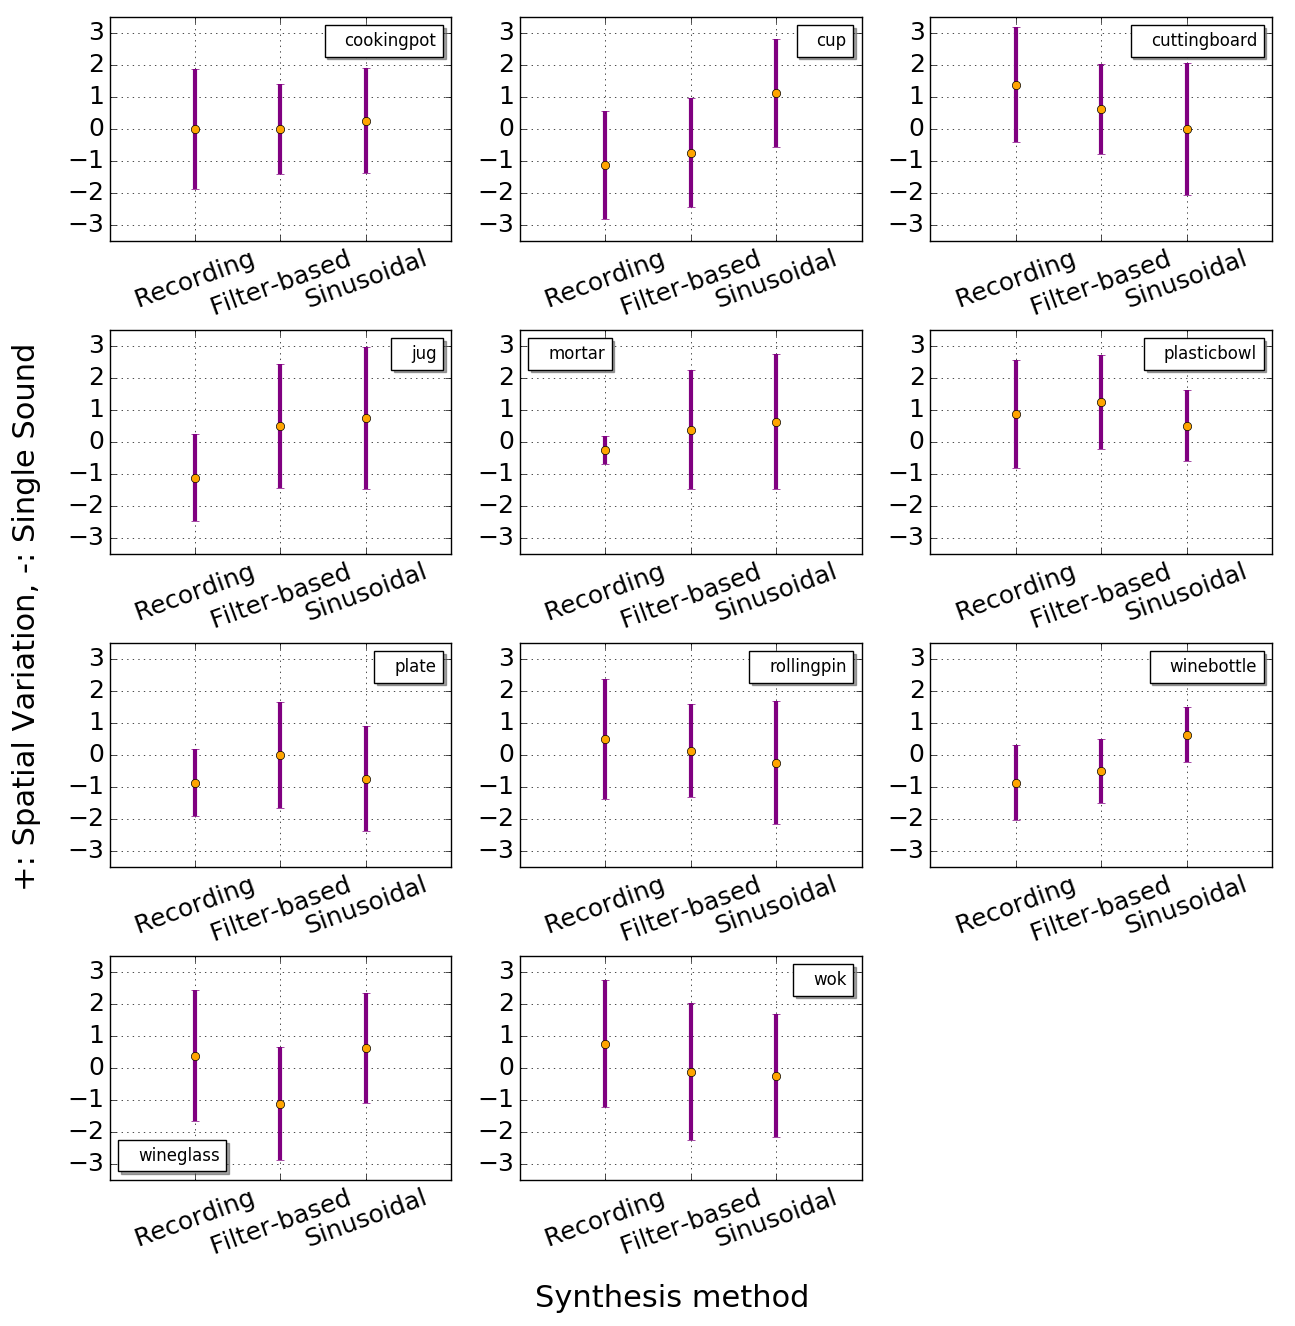
\includegraphics[width=\textwidth]{test2.png}
      \caption{The mean values and standard deviations per location for all objects. Positive values give a preference to the filter-based method, while negative ones give preference to the sinusoidal method. Participants choises were 0: both sound the same, 1/-1: the chosen is slightly better, 2/-2: the chosen is better and 3/-3: the chosen is much better.}\label{fig:test2}
\end{figure}

The aim of this experiment is to prove whether sound variation in game sound effects is desirable and makes a difference. By choosing the positive values, participants would prove that having spatial variation in impact sounds benefits the immersion of the player. \Todo{decribe the graph}

\subsection{3rd experiment}
\Todo{check if it comes out that we cannot transform a given object's material just with damping (maybe we need to change the spectral content)}

Figure \ref{fig:test3} shows the results of the third experiment. This one was held to validate the chosen values of the Q-factor that correspond to each material. For the purpose of this thesis, we chose one value per object that sounded closer to the specified material, in our opinion. Those selected values are shown in table \ref{tab:default_Q}.   

\begin{figure}[H]
  \centering
    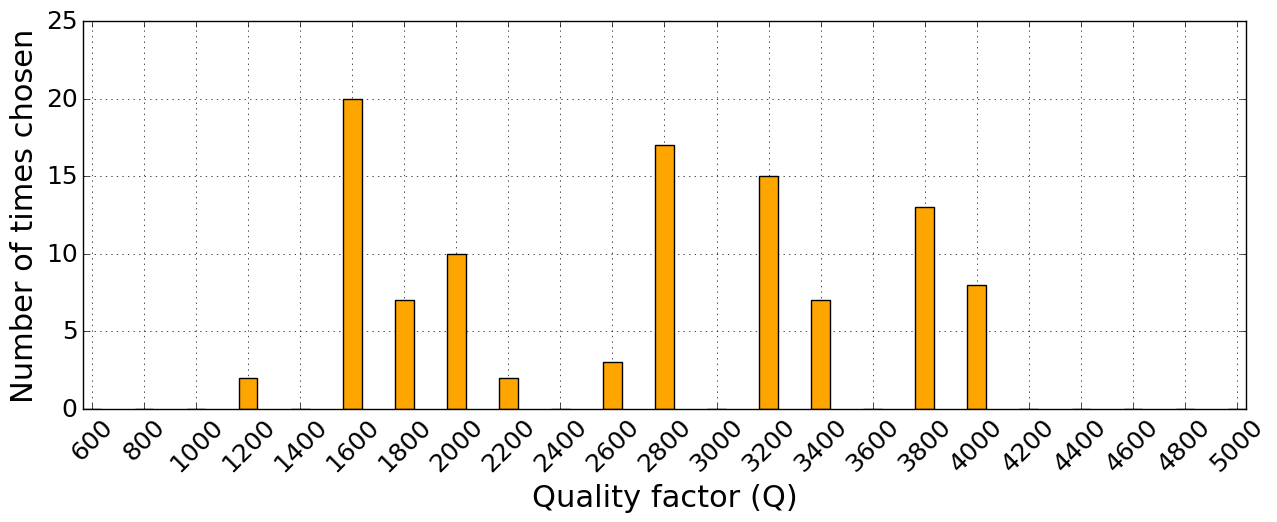
\includegraphics[width=\textwidth]{test3.png}
      \caption{The chosen values of the quality factor that correspond to material change of the same object.}\label{fig:test3}
\end{figure}

By studying figure \ref{fig:test3}, we can see that the values chosen from the experiment participants do not vary a lot from ours.